\section{Specific Requirements}
\subsection{External interface requirements}
\subsubsection{User interfaces}
There are two user interfaces in our system: one for the smartphone used to access the service; one for the onboard infotainment device of the Car.

%
%
%SMARTPHONE UI
%
%
\begin{figure}[h!]
    \centering
    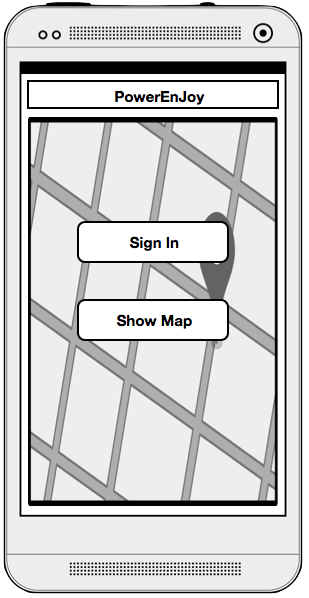
\includegraphics[scale=0.4]{{Figures/Mockup/1FirstScreen.png}}
    \label{fig:1FirstScreen}
    \\Figure 1: From the first screen a user can either sign in, and if necessary create a new account, or consult the map of available Cars.
\end{figure}

\begin{figure}[p!]
    \centering
    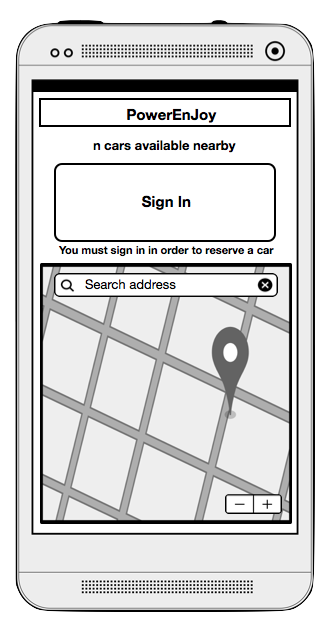
\includegraphics[scale=0.4]{{Figures/Mockup/2MapNotLogged.png}}
    \label{fig:2MapNotLogged}
    \\Figure 2: If a user chooses the map, he will see a map with the positions of all the available Cars; he is asked to sign in in order to proceed with the reservation.
\end{figure}


\begin{figure}[p!]
    \centering
    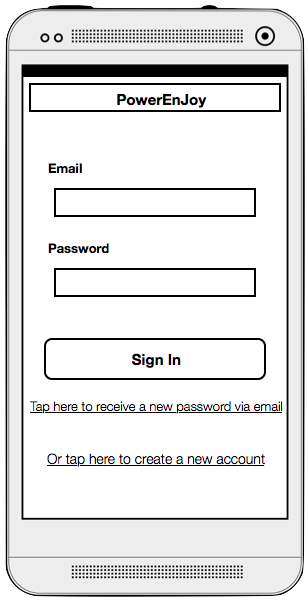
\includegraphics[scale=0.4]{{Figures/Mockup/3LoginForm.png}}
    \label{fig:3LoginForm}
    \\Figure 3: Whether a user started from the map or from the first screen, he will have to either enter his credentials or to register. In case of forgotten credentials he is given the possibility to ask for a new password.
\end{figure}

\begin{figure}[p!]
    \centering
    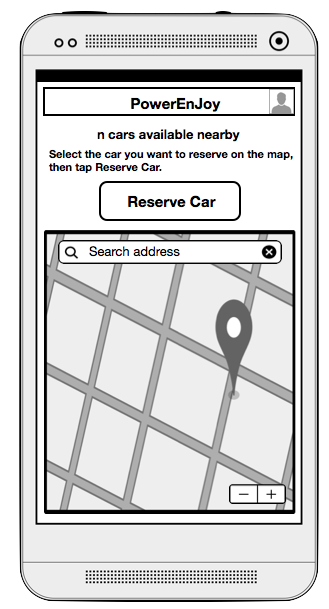
\includegraphics[scale=0.4]{{Figures/Mockup/4CarReservationA}}
    \label{fig:4CarReservationA}
    \\Figure 4: A PowerUser can look for a suitable Car nearby his position or entering an address in the appropriate bar above the map. After finding a Car the PowerUser can select it to know the residual battery and to reserve it.
\end{figure}

\begin{figure}[p!]
    \centering
    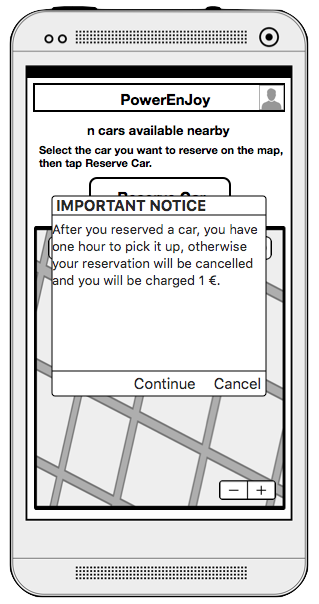
\includegraphics[scale=0.4]{{Figures/Mockup/4CarReservationB.png}}
    \label{fig:4CarReservationB}
    \\Figure 5: Before actually reserving a Car, the system reminds the PowerUser about the one hour expiration of his reservation and the relative penalty fee.
\end{figure}

\begin{figure}[p!]
    \centering
    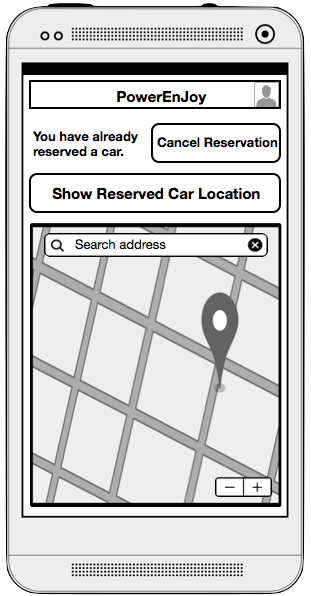
\includegraphics[scale=0.4]{{Figures/Mockup/5CarReserved.png}}
    \label{fig:5CarReserved}
    \\Figure 6: After the selected Car has been reserved, a PowerUser can look for his Car thanks to the provided map or cancel his reservation. In this case a confirmation box pops up before actually cancelling it.
\end{figure}

\begin{figure}[p!]
    \centering
    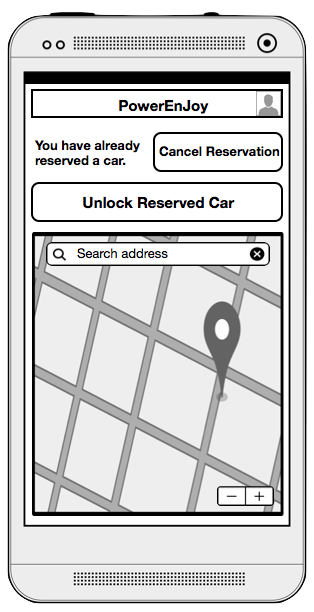
\includegraphics[scale=0.4]{{Figures/Mockup/6CarNearby.png}}
    \label{fig:6CarNearby}
    \\Figure 7: When a PowerUser is near his reserved Car, he is given the possibility to ask the system to unlock it. If the PowerUser changes his mind he can still cancel the reservation, this possibility will remain valid until the PowerUser ignites the engine. 
\end{figure}

\begin{figure}[p!]
    \centering
    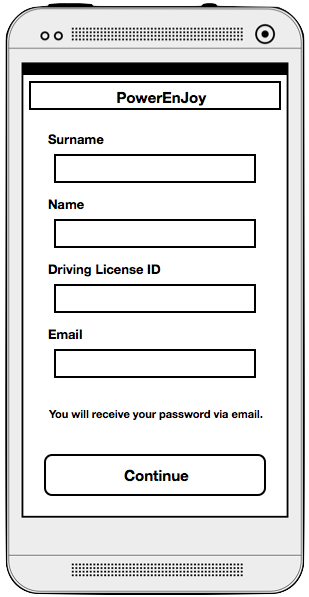
\includegraphics[scale=0.4]{{Figures/Mockup/7RegistrationFormA.png}}
    \label{fig:7RegistrationFormAForm}
    \\Figure 8: This is the first page of the registration procedure; it requires a new user to enter his personal data.
\end{figure}


\begin{figure}[p!]
    \centering
    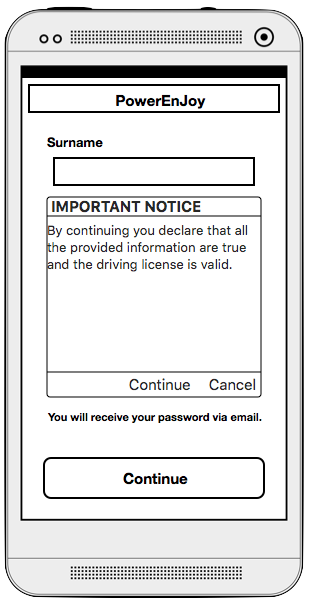
\includegraphics[scale=0.4]{{Figures/Mockup/7RegistrationFormB.png}}
    \label{fig:7RegistrationFormB}
    \\Figure 9: After entering persona data the user is required to provide his driving license details and to accept the Privacy Agreement.
\end{figure}

\begin{figure}[p!]
    \centering
    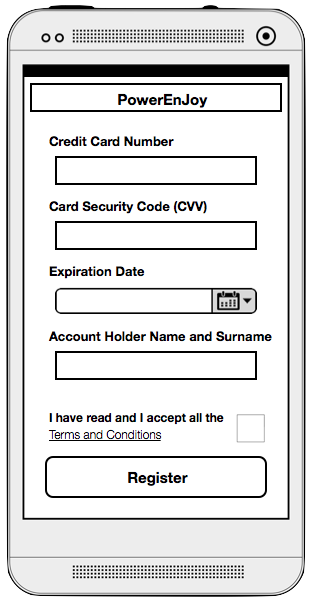
\includegraphics[scale=0.4]{{Figures/Mockup/7RegistrationFormC.png}}
    \label{fig:7RegistrationFormCnForm}
    \\Figure 10: Last page of the registration procedure, the user is asked for his payment information. Furthermore he has to accept the Terms and Conditions of the service in order to complete the registration. These Terms and Conditions contain all the legal constraints required by law, and ensure that any misbehaviour perpetrated by a user is his own solely responsibility and cannot be ascribed to the company running the PowerEnJoy sharing service.
\end{figure}

\begin{figure}[p!]
    \centering
    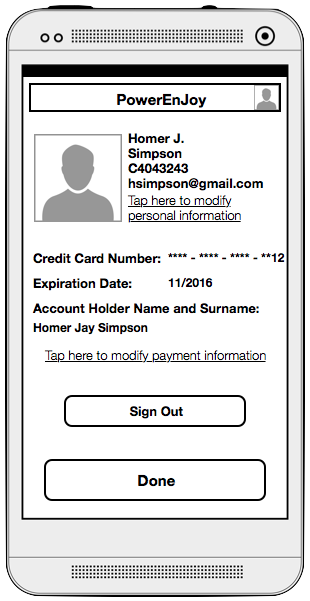
\includegraphics[scale=0.4]{{Figures/Mockup/8PersonalAccountPage.png}}
    \label{fig:8PersonalAccountPage}
    \\Figure 11: A PowerUser can access his personal account page by tapping on the avatar in the top-right corner. By doing so, this is what he will be shown. From this page it is also possible to modify both personal and payment information, or to sign out.
\end{figure}

\begin{figure}[p!]
    \centering
    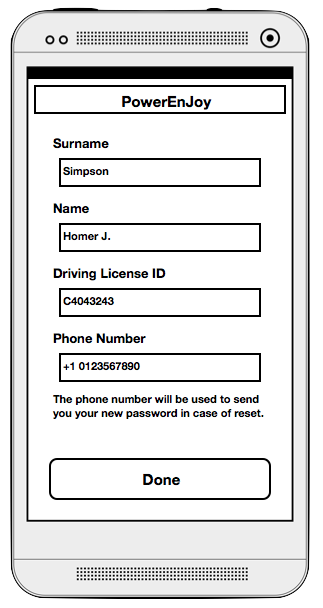
\includegraphics[scale=0.4]{{Figures/Mockup/9PersonalDataModification.png}}
    \label{fig:9PersonalDataModification}
    \\Figure 12: This is the page to be used by a PowerUser in order to modify his personal information.
\end{figure}

\begin{figure}[p!]
    \centering
    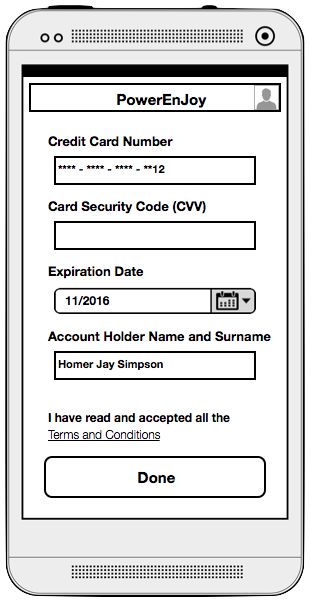
\includegraphics[scale=0.4]{{Figures/Mockup/10PaymentSystemDataModification.png}}
    \label{fig:10PaymentSystemDataModificationForm}
    \\Figure 13: This is the page to be used by a PowerUser in order to modify his payment information.
\end{figure}

%
%
%CAR UI
%
%
\begin{figure}[p!]
    \centering
    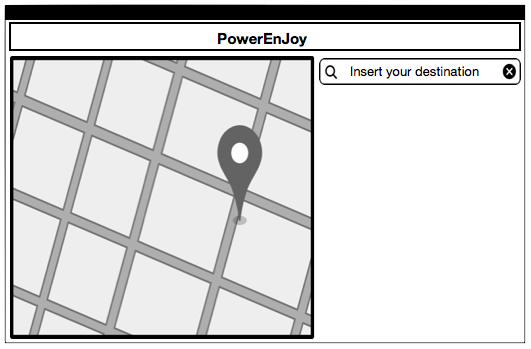
\includegraphics[scale=0.6]{{Figures/Mockup/11FirstCarScreen.png}}
    \label{fig:11FirstCarScreen}
    \\Figure 14: This is the first screen a PowerUser will see entering in a Car. The map on the left is a placeholder for the third party navigation software.
\end{figure}

\begin{figure}[p!]
    \centering
    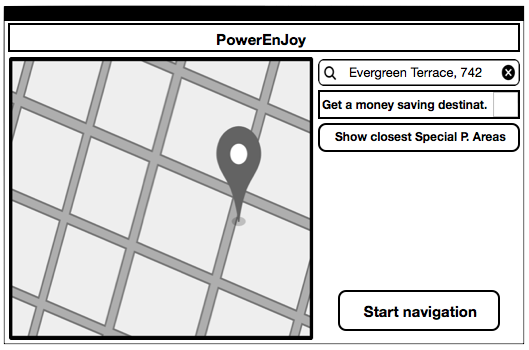
\includegraphics[scale=0.6]{{Figures/Mockup/12aCorrectDestination.png}}
    \label{fig:12aCorrectDestination}
    \\Figure 15: A PowerUser searches for his destination and if it is available in the navigation software he is allowed to start the navigation. Furthermore, he can enable the money saving option using "Get a money saving destination", or ask for the list of the closest Special Parking Areas to his destination.
\end{figure}

\begin{figure}[p!]
    \centering
    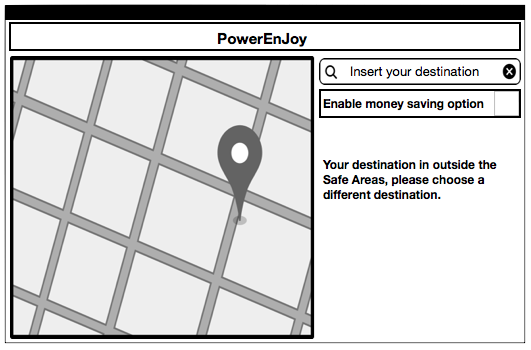
\includegraphics[scale=0.6]{{Figures/Mockup/12bWrongDestination.png}}
    \label{fig:12bWrongDestination}
    \\Figure 16: A PowerUser searches for his destination and if it is not inside the set of Safe Parking Areas he is reminded he cannot park in that position. If he wants he can enable the money saving option using "Get a money saving destination", or ask for the list of the closest Special Parking Areas to his destination.
\end{figure}

\begin{figure}[p!]
    \centering
    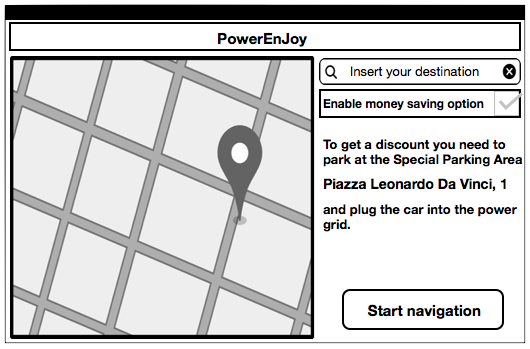
\includegraphics[scale=0.6]{{Figures/Mockup/12cMoneySavingOption.png}}
    \label{fig:12cMoneySavingOption}
    \\Figure 17: When a PowerUser enables the money saving option he is provided with the address of the Special Parking Area where he is supposed to park and plug the car into the power grid in order to get the discount.
\end{figure}

\begin{figure}[p!]
    \centering
    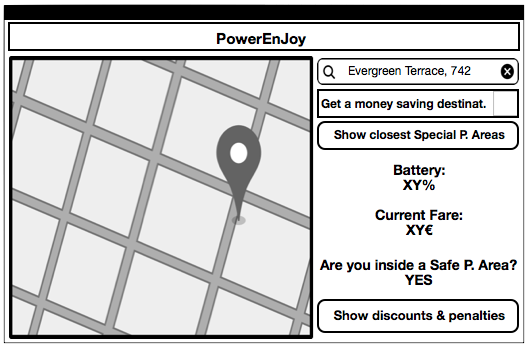
\includegraphics[scale=0.6]{{Figures/Mockup/13Ride.png}}
    \label{fig:13Ride}
    \\Figure 18: This is the screen the PowerUser sees while he is driving. If he needs to change the destination he is free to do that, if he wants to know more about discounts and penalties he can select the apposite button, if he decides to plug the car into the power grid he can ask a money saving destination or the list of the closest Special Parking Areas to his destination.
\end{figure}

\begin{figure}[h!]
    \centering
    \includegraphics[scale=0.6]{{Figures/Mockup/14DiscountsAndPenalties.png}}
    \label{fig:14DiscountsAndPenalties}
    \\Figure 19: This is the screen that sums up all discounts and penalties, and it also declares explicitly which one is valid at the moment. If a PowerUser needs a more detailed description he just have to select the appropriate button to show a window containing all the details and the explanations of each discount and penalty. 
\end{figure}

\newpage

\subsubsection{Hardware interfaces}
The system interfaces directly with sensors and actuators of the Cars, like GPS, door locking and unlocking mechanism, battery sensor, power socket detector.

\subsubsection{Communication interfaces}
The system requires Internet connectivity across all involved devices.

\subsubsection{Software interfaces}
The system relies on a third party payment processor provider to issue payment requests, and a third party navigation software for the onboard Car equipment which provides driving directions.


\subsection{Functional requirements}

\newcounter{goalctr}
    \stepcounter{goalctr}
    \subsubsection{Goal \arabic{goalctr}}
    {[}G\arabic{goalctr}{]}
    Allow any kind of user to view the map of the available nearby Cars.
    \begin{itemize}
        \item Requirements
        \begin{enumerate}[label={[}R\arabic*{]},series=REQ]
    		    \item Users must have access to a map indicating the user current location.
        		\item Users must be able to pan and scroll a map in any direction.
    		    \item Every available Car must be shown on a map.
    	    	\item Users shall have an input for inserting an address in which center the map.
                \item Users shall have an input to center the map view on their position.
        \end{enumerate}
        \item Domain properties
        \begin{enumerate}[label={[}P\arabic*{]},series=PRO]
                \item B\% and C\% are remaining battery power percentages defined during setup.
    			\item No Car with less than B\% battery charge is taken into account as available for booking.
    			\item No Car that is currently under charging and has less than C\% battery charge is taken into account as available for booking.
        \end{enumerate}
    \end{itemize}
    
    \stepcounter{goalctr}
    \subsubsection{Goal \arabic{goalctr}}
    {[}G\arabic{goalctr}{]}
    Allow Visitor user to register to the service.
    \begin{itemize}
        \item Requirements
        \begin{enumerate}[REQ]
    		    \item Let a Visitor user start the registration wizard while he's still not logged in.
			    \item The registration form must contain input fields for user identity, email, contact info, driving license number and expiration, privacy agreement confirmation, credit card number and expiration, billing identity.
			    \item The chosen email address must not be already used by another PowerUser.
			    \item The credit card must be verified not to be blocked or expired upon registration.
			    \item The user must receive a system generated password to the registered email address.
        \end{enumerate}
        \item Domain properties
        \begin{itemize}
    			\item None
        \end{itemize}
    \end{itemize}

    \stepcounter{goalctr}
    \subsubsection{Goal \arabic{goalctr}}
    {[}G\arabic{goalctr}{]}
    Allow Visitor user to log-in and out as a PowerUser.
    \begin{itemize}
        \item Requirements
        \begin{enumerate}[REQ]
			    \item A Visitor user must always see an input to access log-in form as long as he's still not logged in.
		        \item An input to perform log-out must always be available to the PowerUser if he's currently logged in.
        \end{enumerate}
        \item Domain properties
        \begin{itemize}
    			\item None
        \end{itemize}
    \end{itemize}

    \stepcounter{goalctr}
    \subsubsection{Goal \arabic{goalctr}}
    {[}G\arabic{goalctr}{]}
    Allow PowerUser to check the status of the Car.
    \begin{itemize}
        \item Requirements
        \begin{enumerate}[REQ]
    		    \item For each available Car the PowerUser must be able to view its remaining battery charge.
			    \item For each available Car the PowerUser must be able to view its current position.
        \end{enumerate}
        \item Domain properties
        \begin{itemize}
    			\item None
        \end{itemize}
    \end{itemize}

    \stepcounter{goalctr}
    \subsubsection{Goal \arabic{goalctr}}
    {[}G\arabic{goalctr}{]}
    Allow PowerUser to reserve a Car.
    \begin{itemize}
        \item Requirements
        \begin{enumerate}[REQ]
    		    \item The PowerUser must have the ability to start the reservation wizard for all and only available Cars.
			    \item The PowerUser must see a reminder about unfulfilled reservation penalty before confirmation.
			    \item Show an input to allow the PowerUser to confirm and finalize the reservation.
			    \item The system shall prevent the PowerUser to reserve more than a Car from the same geographical region at a time.
        \end{enumerate}
        \item Domain properties
        \begin{enumerate}[PRO]
    			\item Each geographical region has its own set of assigned Cars.
        \end{enumerate}
    \end{itemize}
    
    \stepcounter{goalctr}
    \subsubsection{Goal \arabic{goalctr}}
    {[}G\arabic{goalctr}{]}
    Allow PowerUser to cancel a reservation.
    \begin{itemize}
        \item Requirements
        \begin{enumerate}[REQ]
    			\item If a reservation exists for the PowerUser, show him an input to request cancellation.
    			\item The system shall prompt the PowerUser for cancellation confirmation.
    			\item A reservation must be automatically cancelled by the system after 1 hour from its creation.
    			\item If a reservation is cancelled because of timeout, notify the PowerUser about that occurrence.
        \end{enumerate}
        \item Domain properties
        \begin{itemize}
    			\item None
        \end{itemize}
    \end{itemize}

    \stepcounter{goalctr}
    \subsubsection{Goal \arabic{goalctr}}
    {[}G\arabic{goalctr}{]}
	Allow PowerUser to check the position of the reserved car.
    \begin{itemize}
        \item Requirements
        \begin{enumerate}[REQ]
    	        \item As long as a reservation exists for the PowerUser he must always be able to get the position of the reserved Car on the map.
        \end{enumerate}
        \item Domain properties
        \begin{itemize}
    			\item None
        \end{itemize}
    \end{itemize}

    \stepcounter{goalctr}
    \subsubsection{Goal \arabic{goalctr}}
    {[}G\arabic{goalctr}{]}
	Allow PowerUser to unlock and enter the Car when inside the specific range.
    \begin{itemize}
        \item Requirements
        \begin{enumerate}[REQ]
    	        \item The system must be able to remotely unlock the Car.
			    \item The system must be able to compute the distance between the user location and his reserved Car.
			    \item The PowerUser must have an input allowing him to send an unlock request.
			    \item The system must accept the unlock request issued by the PowerUser if and only if the PowerUser is in the unlock allowance area.
			    \item If the unlock request is accepted, the PowerUser must be able to enter the Car.
        \end{enumerate}
        \item Domain properties
        \begin{enumerate}[PRO]
                \item The PowerUser position is always the same as of its mobile device that runs the PowerUser application.
    			\item The PowerUser is considered to be in the unlocking allowance area if the distance to the Car is at most equal to 5 meters.
        \end{enumerate}
    \end{itemize}
    
    \stepcounter{goalctr}
    \subsubsection{Goal \arabic{goalctr}}
    {[}G\arabic{goalctr}{]}
    Allow PowerUser to get driving directions to his destination.
    \begin{itemize}
        \item Requirements
        \begin{enumerate}[REQ]
    			\item The user must be allowed to select a custom destination and start navigating to that location.
        \end{enumerate}
        \item Domain properties
        \begin{enumerate}[PRO]
    			\item Navigation software always provides effective directions to the user if the destination is included in the Safe Parking Areas.
        \end{enumerate}
    \end{itemize}
    
    \stepcounter{goalctr}
    \subsubsection{Goal \arabic{goalctr}}
    {[}G\arabic{goalctr}{]}
	Bill the PowerUser for the amount of time spent riding a Car.
    \begin{itemize}
        \item Requirements
        \begin{enumerate}[REQ]
                \item Start counting the billing time from the first engine ignition.
    	        \item Stop the billing time counter exactly 1 second after the Car locking.
        \end{enumerate}
        \item Domain properties
        \begin{itemize}
    			\item None
        \end{itemize}
    \end{itemize}

    \stepcounter{goalctr}
    \subsubsection{Goal \arabic{goalctr}}
    {[}G\arabic{goalctr}{]}
    Allow PowerUser to see a list of the closest Special Parking Areas to his destination.
    \begin{itemize}
        \item Requirements
        \begin{enumerate}[REQ]
    		    \item The system must be capable of providing a list of Special Parking Areas sorted by distance from an input location.
			    \item PowerUser must be allowed anytime during the navigation to input a custom location and be acknowledged about all nearest Special Parking Areas from the selected location.
        \end{enumerate}
        \item Domain properties
        \begin{itemize}
    			\item None
        \end{itemize}
    \end{itemize}
    
    \stepcounter{goalctr}
    \subsubsection{Goal \arabic{goalctr}}
    {[}G\arabic{goalctr}{]}
    Allow PowerUser to keep track of the Current Fare.
    \begin{itemize}
        \item Requirements
        \begin{enumerate}[REQ]
    			\item Show on the Car screen a live updated counter indicating the Current Fare amount that the user would actually pay if the ride ended in that same moment, as long as the ride is being charged.
        \end{enumerate}
        \item Domain properties
        \begin{enumerate}[PRO]
    			\item The Current Fare starts being counted when the engine ignites for the first time and stops exactly 1 second after the Car locking.
        \end{enumerate}
    \end{itemize}
    
    \stepcounter{goalctr}
    \subsubsection{Goal \arabic{goalctr}}
    {[}G\arabic{goalctr}{]}
    Allow PowerUser to check whether he can be eligible for any discount or penalty.
    \begin{itemize}
        \item Requirements
        \begin{enumerate}[REQ]
    			\item Provide through Car screen an input to access an overview of all discounts and penalties.
    			\item For each shown discount or penalty allow the PowerUser to get a brief informal description of corresponding criteria.
    			\item For each shown discount or penalty allow the PowerUser to know if the current ride satisfies all needed criteria at the moment.
        \end{enumerate}
        \item Domain properties
        \begin{itemize}
    			\item None
        \end{itemize}
    \end{itemize}
 
    \stepcounter{goalctr}
    \subsubsection{Goal \arabic{goalctr}}
    {[}G\arabic{goalctr}{]}
    Allow PowerUser to get a money saving alternative destination.
    \begin{itemize}
        \item Requirements
        \begin{enumerate}[REQ]
    			\item Show the PowerUser the option to get a money saving destination alternative after entering desired destination address.
    			\item Always show to PowerUser an input to get money saving proposal even if there already exists a selected destination.
    			\item The destination proposal must correspond to the nearest (w.r.t. PowerUser selected destination) Special Parking Area where there are less than N\# Cars attached to the power source.
    			\item If the PowerUser accepts the money saving destination proposal, the current selected destination must be updated accordingly.
        \end{enumerate}
        \item Domain properties
        \begin{enumerate}[PRO]
                \item N\# is an integer number defined during setup.
    			\item Special Parking Areas provide at least N\# power sockets as exclusively available to PowerEnJoy customers.
        \end{enumerate}
    \end{itemize}
 
    \stepcounter{goalctr}
    \subsubsection{Goal \arabic{goalctr}}
    {[}G\arabic{goalctr}{]}
    Allow the system to lock the Car in a Safe Parking Area at the end of the ride.
    \begin{itemize}
        \item Requirements
        \begin{enumerate}[REQ]
    			\item The system must lock the Car if its position belong to the set of Safe Parking Areas, engine is stopped, all doors are closed and S\# seconds passed from the last door closure.
        \end{enumerate}
        \item Domain properties
        \begin{enumerate}[PRO]
                \item S\# is a time-span defined during setup.
    			\item At least a free parking slot is available for the user among all Safe Parking Areas.
        \end{enumerate}
    \end{itemize} 
 
    \stepcounter{goalctr}
    \subsubsection{Goal \arabic{goalctr}}
    {[}G\arabic{goalctr}{]}
    Allow the system to apply penalty or discount according to the given criteria.
    \begin{itemize}
        \item Requirements
        \begin{enumerate}[REQ]
    			\item The system shall apply a discount of 10\% on the last ride Total Base Fare if the number of passengers at the end of the ride is greater or equal to the number of passengers at the start of the ride and the number of passengers at the start of the ride was at least 3, driver included.
    			\item The system shall apply a discount of 20\% on the last ride Total Base Fare if the remaining battery power at the end of the ride is greater or equal then 50\%.
    			\item The system shall apply a discount of 30\% on the last ride Total Base Fare if the Car position at the end of the ride is within a Special Parking Areas and the power socket is detected as connected two minutes from the Car locking.
    			\item The system shall apply a penalty of 30\% on the last ride Total Base Fare if the position of the Car at the time of locking is more than 3km far from the nearest power grid station, or the remaining battery power is less than 20\% and the Car is not detected as attached to power grid within two minutes from locking.
        \end{enumerate}
        \item Domain properties
        \begin{itemize}
    			\item None
        \end{itemize}
    \end{itemize} 

    \stepcounter{goalctr}
    \subsubsection{Goal \arabic{goalctr}}
    {[}G\arabic{goalctr}{]}
    Let the system bill the PowerUser for the Total Ride Fare and issue a payment request for that amount at the end of the ride.
    \begin{itemize}
        \item Requirements
        \begin{enumerate}[REQ]
    			\item The system must charge the PowerUser the Total Ride Fare after two minutes and an half from the Car locking.
    			\item The system must issue the payment request to the Payment Processor Provider.	
    			\item The system must bill the PowerUser a penalty of 1$\euro$ as soon as a reservation he made expires by timeout.
    			\item The PowerUser shall be notified of any money charge by email.
    			\item The PowerUser shall be notified of the payment transaction result.
        \end{enumerate}
        \item Domain properties
        \begin{itemize}
    			\item None
        \end{itemize}
    \end{itemize}


\newpage
\subsection{Use cases}

\begin{figure}[h!]
    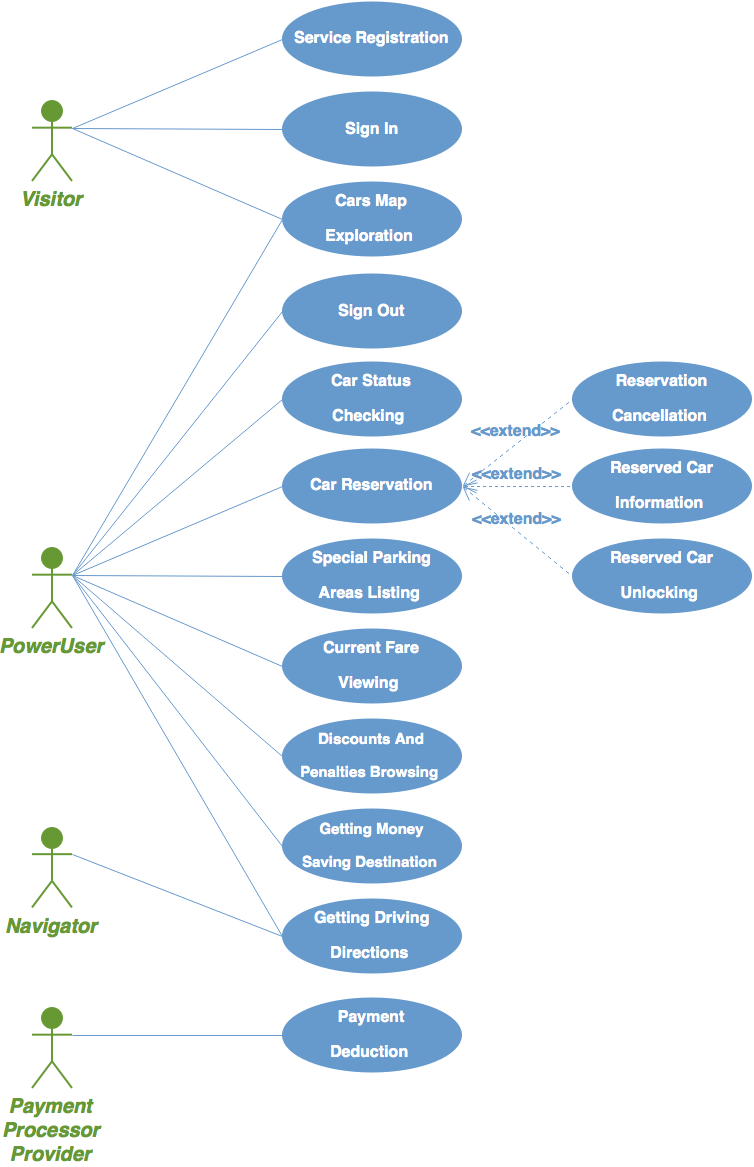
\includegraphics[scale=0.45]{{Figures/UseCaseDiagram.png}}
    \label{fig:UseCaseDiagram}
    \newline
    A use case \textit{extends} another use case when its use is optional and the use case that is extended is already reasonably complete.
\end{figure}


\newpage
\subsubsection{Cars Map Exploration}
\begin{tabular}{| l | p{10cm} |}
\hline
\textbf{Actor}      &       Visitor, PowerUser \\
\hline
\textbf{Goal}       &       [G1]\\
\hline
\textbf{Entry Condition} &  NULL\\
\hline
\textbf{Event Flow}     &   1.	The user launches the application.\\&
                            2.  He taps on "Show Map".\\&
                            3.  He sees a map with the available Cars.\\&
                            4.	He sees a pointer corresponding to his current position.\\&
                            5.  He scrolls the map in any direction.\\
\hline
\textbf{Output Condition} & NULL\\
\hline
\textbf{Exceptions} &       ?   Cannot obtain current position.\\& 
                           The exception is handled notifying the user about the exception.\\
\hline
\end{tabular} 
\begin{figure}[h!]
    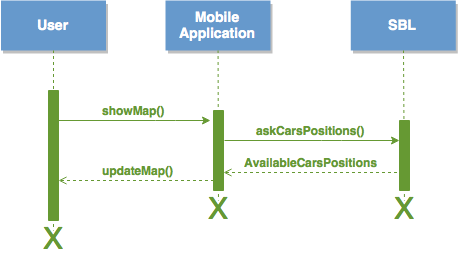
\includegraphics[scale=0.6]{{Figures/SequenceDiagram/1CarMapExploration.png}}
    \label{fig:1CarMapExploration}
\end{figure}


\newpage
\subsubsection{Service Registration}
\begin{tabular}{| l | p{10cm} |}
\hline
\textbf{Actor}      &       Visitor \\
\hline
\textbf{Goal}       &       [G2]\\
\hline
\textbf{Entry Condition} &  NULL\\
\hline
\textbf{Event Flow}     &   1.	Visitor launches
the application.\\&
                        2. He accesses the Sign In view.\\&
                        3. He taps on the apposite string to create a new account.\\&
                                            3.	He compiles all required fields.\\&
                                            4.	The system sends the password to the specified email.\\
\hline
\textbf{Output Condition} & A new PoweUser account exists.\\
\hline
\textbf{Exceptions} &       ?   Input fields validation failure.\\& 
                            ?	Cannot send email to selected address.\\&
                           These exceptions are handled notifying the user about the exception, asking him to give new valid/working inputs.\\
\hline
\end{tabular} 
\begin{figure}[h!]
    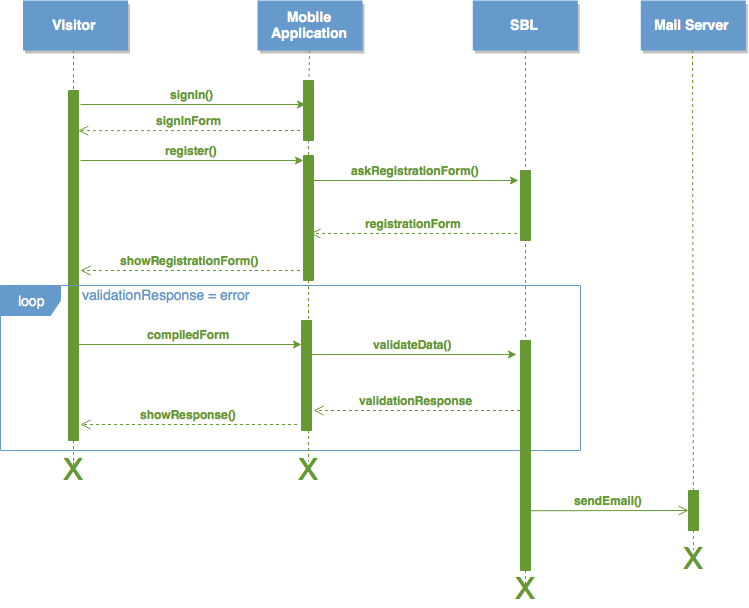
\includegraphics[scale=0.6]{{Figures/SequenceDiagram/2ServiceRegistration.png}}
    \label{fig:2ServiceRegistration}
\end{figure}


\newpage
\subsubsection{Sign In}
\begin{tabular}{| l | p{10cm} |}
\hline
\textbf{Actor}      &       Visitor \\
\hline
\textbf{Goal}       &       [G3]\\
\hline
\textbf{Entry Condition} &  NULL\\
\hline
\textbf{Event Flow}     &   1.	Visitor reaches the Sign In page.\\&
                        2. He inputs his PowerUser's email address and his Power-User's password.\\&
                        3. He confirms tapping the "Sign In" button.\\
\hline
\textbf{Output Condition} & Visitor is now authenticated as a PowerUser.\\
\hline
\textbf{Exceptions} &       ?   Wrong credentials.\\&
                           The exception is handled notifying the user about the exception, asking him to check for errors in given credentials.\\
\hline
\end{tabular} 
\begin{figure}[h!]
    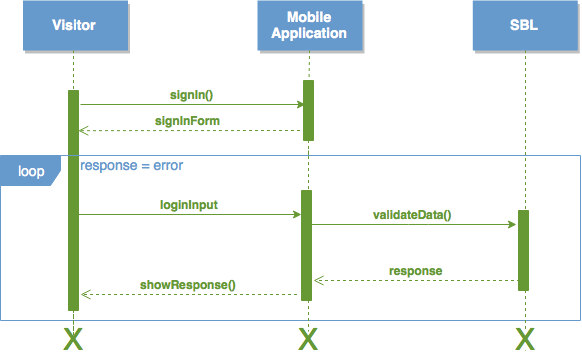
\includegraphics[scale=0.6]{{Figures/SequenceDiagram/3SignIn.png}}
    \label{fig:3SignIn}
\end{figure}


\newpage
\subsubsection{Sign Out}
\begin{tabular}{| l | p{10cm} |}
\hline
\textbf{Actor}      &       PowerUser \\
\hline
\textbf{Goal}       &       [G3]\\
\hline
\textbf{Entry Condition} &  Existent PowerUser authenticated session.\\
\hline
\textbf{Event Flow}     &   1.	PowerUser reaches his personal page.\\&
2. He taps on the "Sign Out" button to deactivate the current signed-in session.\\
\hline
\textbf{Output Condition} & PowerUser is no more recognized as such, until he signs in again.\\
\hline
\textbf{Exceptions} &       NONE\\
\hline
\end{tabular} 
\begin{figure}[h!]
    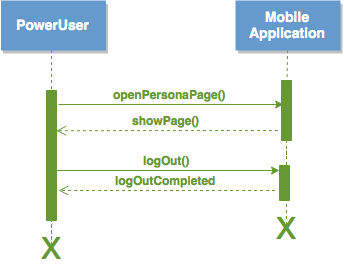
\includegraphics[scale=0.6]{{Figures/SequenceDiagram/4SignOut.png}}
    \label{fig:4SignOut}
\end{figure}


\newpage
\subsubsection{Car Status Checking}
\begin{tabular}{| l | p{10cm} |}
\hline
\textbf{Actor}      &       PowerUser \\
\hline
\textbf{Goal}       &       [G4]\\
\hline
\textbf{Entry Condition} &  A Car is shown on the map.\\
\hline
\textbf{Event Flow}     &   1.	The PowerUser selects an available Car on the map.\\&
                            2.	He gets details about the remaining battery charge.\\
\hline
\textbf{Output Condition} & PowerUser sees an input to proceed reserving that Car.\\
\hline
\textbf{Exceptions} &       NONE\\
\hline
\end{tabular} 
\begin{figure}[h!]
    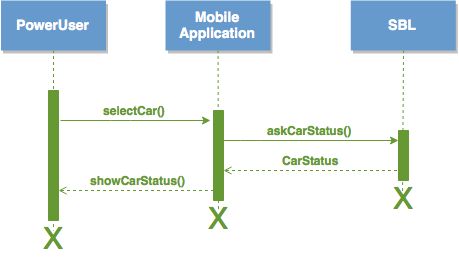
\includegraphics[scale=0.6]{{Figures/SequenceDiagram/5CarStatusChecking.png}}
    \label{fig:5CarStatusChecking}
\end{figure}


\newpage
\subsubsection{Car Reservation}
\begin{tabular}{| l | p{10cm} |}
\hline
\textbf{Actor}      &       PowerUser \\
\hline
\textbf{Goal}       &       [G5]\\
\hline
\textbf{Entry Condition} &  PowerUser has no other active reservation.\\
\hline
\textbf{Event Flow}     &   1.	PowerUser starts the reservation wizard.\\&
                            2.	He sees a warning about reservation cancellation timeout.\\&
                            3.	He accepts to continue reserving the Car.\\&
                            4.  He sees a timer to the time of reservation expiration.\\
\hline
\textbf{Output Condition} & PowerUser has a pending reservation for the selected Car.\\
\hline
\textbf{Exceptions} &       ?   Car no longer available.\\& 
                           The exception is handled notifying the user about the exception, asking him to choose another Car.\\
\hline
\end{tabular} 
\begin{figure}[h!]
    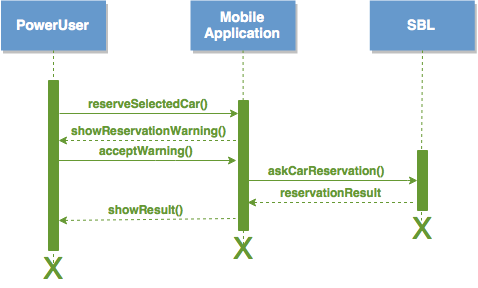
\includegraphics[scale=0.6]{{Figures/SequenceDiagram/6CarReservation.png}}
    \label{fig:6CarReservation}
\end{figure}


\newpage
\subsubsection{Reservation Cancellation}
\begin{tabular}{| l | p{10cm} |}
\hline
\textbf{Actor}      &       PowerUser \\
\hline
\textbf{Goal}       &       [G6]\\
\hline
\textbf{Entry Condition} &  Existent pending Car reservation for PowerUser.\\
\hline
\textbf{Event Flow}     &   1.	PowerUser asks to cancel the current pending reservation.\\&
                            2. He sees a confirmation message.\\&
                            3.	He accepts to continue cancelling the reservation.\\
\hline
\textbf{Output Condition} & PowerUser has no pending Car reservation.\\
\hline
\textbf{Exceptions} &       ?   Reservation expired meanwhile.\\&
                           The exception is handled aborting the cancellation wizard.\\
\hline
\end{tabular} 
\begin{figure}[h!]
    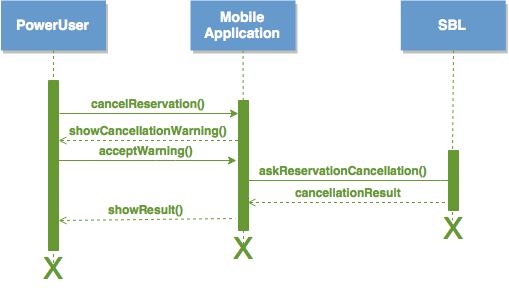
\includegraphics[scale=0.6]{{Figures/SequenceDiagram/7ReservationCancellation.png}}
    \label{fig:7ReservationCancellation}
\end{figure}


\newpage
\subsubsection{Reserved Car Information}
\begin{tabular}{| l | p{10cm} |}
\hline
\textbf{Actor}      &       PowerUser \\
\hline
\textbf{Goal}       &       [G7]\\
\hline
\textbf{Entry Condition} &  Existent pending Car reservation for PowerUser.\\
\hline
\textbf{Event Flow}     &   1.	PowerUser asks to show the reserved Car on the map.\\&
                            2.	He sees the Car on the map with its remaining battery charge.\\
\hline
\textbf{Output Condition} & NULL\\
\hline
\textbf{Exceptions} &       NONE\\
\hline
\end{tabular} 
\begin{figure}[h!]
    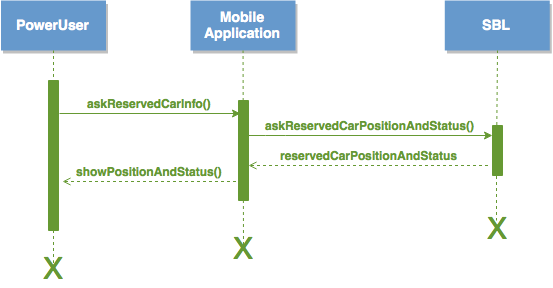
\includegraphics[scale=0.6]{{Figures/SequenceDiagram/8ReservedCarInformation.png}}
    \label{fig:8ReservedCarInformation}
\end{figure}


\newpage
\subsubsection{Reserved Car Unlocking}
\begin{tabular}{| l | p{10cm} |}
\hline
\textbf{Actor}      &       PowerUser \\
\hline
\textbf{Goal}       &       [G8]\\
\hline
\textbf{Entry Condition} &  Existent pending Car reservation for PowerUser and PowerUser is inside the allowed unlocking area.\\
\hline
\textbf{Event Flow}     &   1.	PowerUser sees an option to unlock the reserved Car.\\&
                            2.	He asks the Car to be unlocked.\\&
                            3.	The system unlocks the Car.\\&
                            4.  PowerUser opens the door and enters the Car.\\
\hline
\textbf{Output Condition} & Car doors are unlocked.\\
\hline
\textbf{Exceptions} &       ?   Unable to unlock the Car.\\& 
                           The exception is handled asking the PowerUser to retry in a few seconds.\\
\hline
\end{tabular} 
\begin{figure}[h!]
    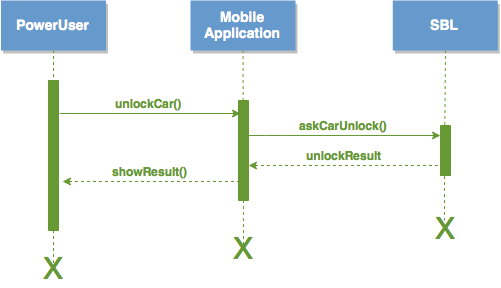
\includegraphics[scale=0.6]{{Figures/SequenceDiagram/9ReservedCarUnlocking.png}}
    \label{fig:9ReservedCarUnlocking}
\end{figure}


\newpage
\subsubsection{Getting Driving Directions}
\begin{tabular}{| l | p{10cm} |}
\hline
\textbf{Actor}      &       PowerUser, Navigator \\
\hline
\textbf{Goal}       &       [G9]\\
\hline
\textbf{Entry Condition} &  There exists a selected destination.\\
\hline
\textbf{Event Flow}     &   1.	PowerUser chooses to start navigation in order to be given directions by the onboard navigator for the previously selected destination.\\&
                            2.	He follows the directions.\\
\hline
\textbf{Output Condition} & The destination is reached.\\
\hline
\textbf{Exceptions} &       ?	Cannot find driving direction for selected destination.\\& 
                           The exception is handled asking the PowerUser to select another destination to get driving directions to which is surely reachable by car.\\
\hline
\end{tabular} 
\begin{figure}[h!]
    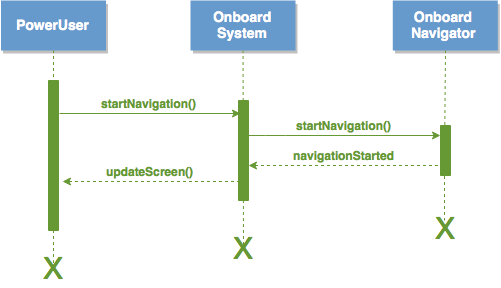
\includegraphics[scale=0.6]{{Figures/SequenceDiagram/10GettingDrivingDirections.png}}
    \label{fig:10GettingDrivingDirections}
\end{figure}


\newpage
\subsubsection{Special Parking Areas Listing}
\begin{tabular}{| l | p{10cm} |}
\hline
\textbf{Actor}      &       PowerUser \\
\hline
\textbf{Goal}       &       [G11]\\
\hline
\textbf{Entry Condition} &  There exists a selected destination.\\
\hline
\textbf{Event Flow}     &   1.	PowerUser asks for a list of Special Parking Areas.\\&
                            2.	The system lets him scroll a list of Special parking Areas sorted by distance to his selected destination.\\&
                            3.	PowerUser optionally selects one of those as new destination.\\
\hline
\textbf{Output Condition} & NULL or current selected destination changed.\\
\hline
\textbf{Exceptions} &       NONE\\
\hline
\end{tabular} 
\begin{figure}[h!]
    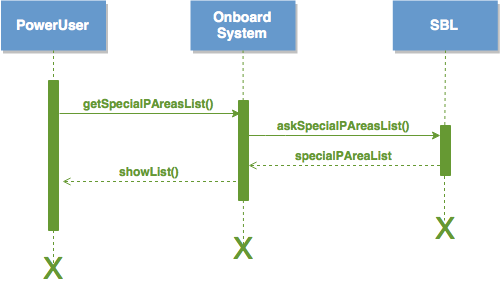
\includegraphics[scale=0.6]{{Figures/SequenceDiagram/11SpecialParkingAreasListing.png}}
    \label{fig:11SpecialParkingAreasListing}
\end{figure}


\newpage
\subsubsection{Current Fare Viewing}
\begin{tabular}{| l | p{10cm} |}
\hline
\textbf{Actor}      &       PowerUser \\
\hline
\textbf{Goal}       &       [G12]\\
\hline
\textbf{Entry Condition} &  Ride is being currently charged.\\
\hline
\textbf{Event Flow}     &   1.	PowerUser sees the updated Current Fare amount on the onboard screen of the Car.\\
\hline
\textbf{Output Condition} & NULL\\
\hline
\textbf{Exceptions} &       NONE\\
\hline
\end{tabular} 
\begin{figure}[h!]
    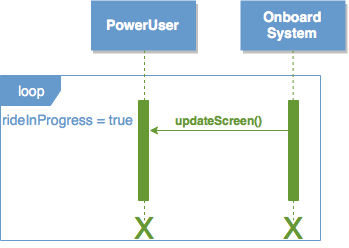
\includegraphics[scale=0.6]{{Figures/SequenceDiagram/12CurrentChargedFareViewing.png}}
    \label{fig:12CurrentChargedFareViewing}
\end{figure}


\newpage
\subsubsection{Discounts And Penalties Browsing}
\begin{tabular}{| l | p{10cm} |}
\hline
\textbf{Actor}      &       PowerUser \\
\hline
\textbf{Goal}       &       [G13]\\
\hline
\textbf{Entry Condition} &  NULL\\
\hline
\textbf{Event Flow}     &   1.	PowerUser opens the discounts and penalties lists.\\&
                            2.	He gets the lists of all existing available discounts and penalties policies.\\&
                            3.  He gets a visible feedback stating if those criteria yield for the current ride.\\&
                            4.	At the end of the lists he can ask for a detailed description.\\
\hline
\textbf{Output Condition} & NULL\\
\hline
\textbf{Exceptions} &      NONE\\
\hline
\end{tabular} 
\begin{figure}[h!]
    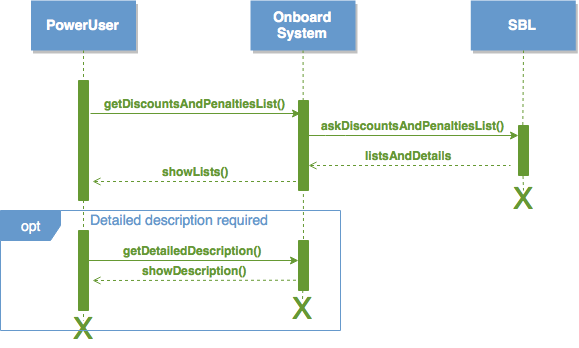
\includegraphics[scale=0.6]{{Figures/SequenceDiagram/13DiscountsAndPenaltiesBrowsing.png}}
    \label{fig:13DiscountsAndPenaltiesBrowsing}
\end{figure}


\newpage
\subsubsection{Getting Money Saving Destination}
\begin{tabular}{| l | p{10cm} |}
\hline
\textbf{Actor}      &       PowerUser \\
\hline
\textbf{Goal}       &       [G14]\\
\hline
\textbf{Entry Condition} &  A destination is being selected or there already exists one.\\
\hline
\textbf{Event Flow}     &   1.	PowerUsers enables the Money Saving destination.\\&
                            2.	The system provides him a single Special Parking Area and its location on a map.\\&
                            3.	PowerUser either accepts the proposal by starting the navigation or rejects it by disabling the Money Saving destination.\\&
                            4.  If accepted, the selected destination is updated accordingly.\\
\hline
\textbf{Output Condition} & Suggested proposal rejected or accepted.\\
\hline
\textbf{Exceptions} &       NONE\\
\hline
\end{tabular} 
\begin{figure}[h!]
    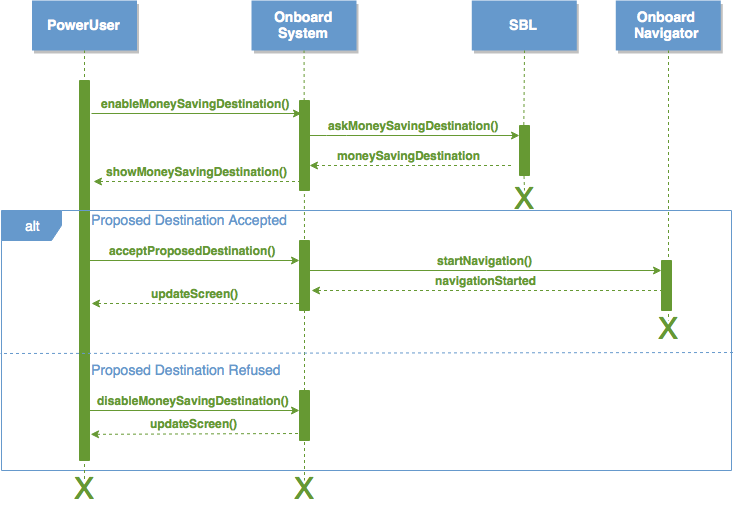
\includegraphics[scale=0.6]{{Figures/SequenceDiagram/14MoneySavingSuggestion.png}}
    \label{fig:14MoneySavingSuggestion}
\end{figure}


\newpage
\subsubsection{Payment Deduction}
\begin{tabular}{| l | p{10cm} |}
\hline
\textbf{Actor}      &       Payment Processor Provider \\
\hline
\textbf{Goal}       &       [G17]\\
\hline
\textbf{Entry Condition} &  Locking grace period expired.\\
\hline
\textbf{Event Flow}     &   1.	The system locks the Car and stops charging the PowerUser.\\&
                            2.	The system creates a new payment request for the ride just ended.\\&
                            3.	The system merges it with all pending payments for penalties or previous rides of the same account into a single comprehensive payment request.\\&
                            2.	The system issues the payment request to the PPP.\\&
                            3.	PPP responds back with operation result and transaction details.\\&
                            4.  The system sends an email to the PowerUser with payment result and details.\\
\hline
\textbf{Output Condition} & The amount of money has been transferred from PowerUser to PEJ.\\
\hline
\textbf{Exceptions} &       ?   Not enough money.\\&
                           The exception is handled notifying the user of the issue and adding that payment request to the pending ones.\\
\hline
\end{tabular} 
\begin{figure}[h!]
    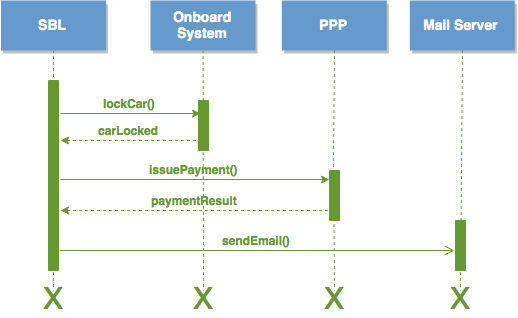
\includegraphics[scale=0.6]{{Figures/SequenceDiagram/15PaymentDeduction.png}}
    \label{fig:15PaymentDeduction}
\end{figure}